\section{Analysis}\label{sec:analysis}

    \subsection{Data and noise}\label{sec:data}
        The function, onto which we are trying to fit a model, is the Franke function. It is defined as follows:
        \begin{align}\label{eq:francefunc}
            f(x,y) &= \frac{3}{4}\exp{-\frac{(9x-2)^2}{4}-\frac{(9y-2)^2}{4}} \nonumber\\
            &+ \frac{3}{4}\exp{-\frac{(9x+1)^2}{49}-\frac{(9y+1)}{10}} \nonumber\\
            &+ \frac{1}{2}\exp{-\frac{(9x-7)^2}{4}-\frac{(9y-3)^2}{4}} \nonumber\\
            &-\frac{1}{5}\exp{-(9x-4)^2-(9y-7)^2}.
        \end{align}
        In order to generate a dataset we will use $N$ uniformly distributed values of $x,y\in[0,1]$. We will also add some normally distributed noise $\epsilon = \eta\mathcal{N}(\mu,\sigma^2) = \eta\mathcal{N}(0,1)$ to $f(x,y)$, where $\eta$ is a strength parameter controlling the amplitude of the added noise. The full description of our data then become:
        \begin{align}\label{eq:datadescription}
            \vec{y} &= f(x,y) + \eta\mathcal{N}(0,1) \nonumber \\
            &= f(\vec{x}) + \epsilon
        \end{align}
        where $\vec{x} = (x,y)$. 
        From section \Sec{regression} we have a model for this data: $\tilde{\vec{y}} = X\hat{\svec{\beta}}$ where $X$ is the design matrix and $\hat{\svec{\beta}}$ are the optimal parameters which we are trying to determine. 

        We visualise the data both with and without noise. \Fig{franke_function} shows the Franke function without any noise ($\eta=0$), plotted for uniformly distributed $x$ and $y$, where $N=20$. We could use more data points, but for the sake computational efficiency we use a $20\cross20$ grid throughout this analysis. \Fig{franke_function_noise} shows the same function, for the same points but now with an added noise of amplitude $\eta=0.1$.

        \begin{figure}
            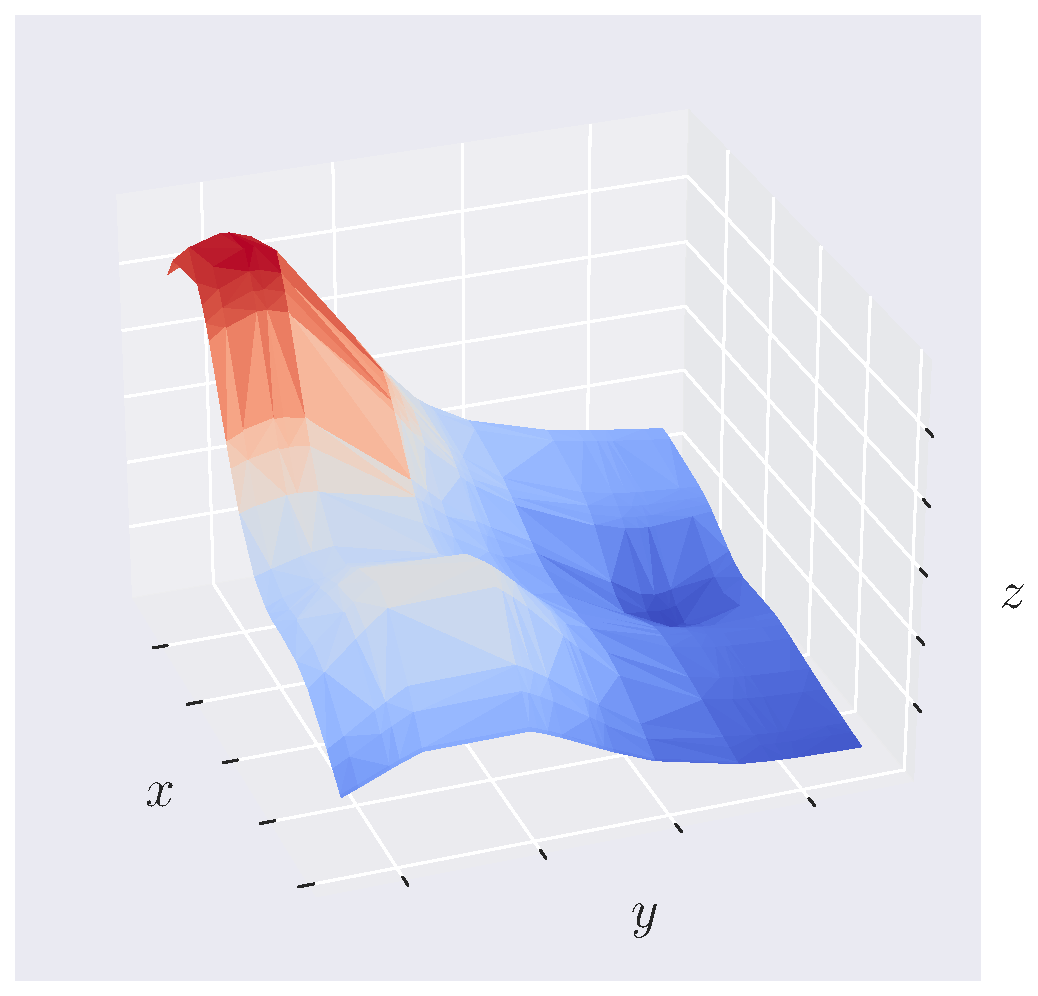
\includegraphics[width=\linewidth]{Franke/data3D_no_noise.pdf}
            \caption{The Franke function plotted on a grid where $N=20$ and $\eta=0$. Since we scale the data, the $z$-values become arbitrary and we choose to leave them out. The important information is the shape of the graph which is smooth when there is no noise. }
            \label{fig:franke_function}
        \end{figure}

        \begin{figure}
            \includegraphics[width=\linewidth]{Franke/data3D.pdf}
            \caption{The Franke function with added noise plotted on a grid where $N=20$ and $\eta=0.1$. Since we scale the data, the $z$-values become arbitrary and we choose to leave them out. The important information is the shape of the graph which becomes quite ragged even for this small level of noise.}
            \label{fig:franke_function_noise}
        \end{figure}

    \subsection{Data splitting}\label{sec:splitting}
        In order to test our estimate of $\hat{\svec{\beta}}$ we reserve some of the data for testing. We thus divide our data set into a part for testing a part for training. We select 80 \% of the data for training and the remaining 20 \% for testing the data. The data is split at random. 




    \subsection{Model and design matrix}\label{sec:model}
        The design matrix $X$ has dimensionality ($n\cross p$) where $n$ represents the data points and $p$ the features of the model. We have already split the data set into training and testing, and must therefore create two design matrices: $X^{\text{train}}$ and $X^{\text{test}}$. 
        \\
        We want our model to be a two-dimensional polynomial of order $d$:
        %P_d(x,y) = \beta_0 + \sum_{l=1}^d\sum_{k=0}^{l} \beta_jx^{l-k}y^k \\
        \begin{align*}
            P_d(x,y) =& \beta_0 + \beta_1 x + \beta_2 y + \beta_3 x^2 + \beta_4 xy + \beta_5 y^2 + \dots \\
            &+ \beta_{p-d-1} x^d + \beta_{p-d} x^{d-1}y + \dots + \beta_p y^d,
        \end{align*}
        where $j\in[1,p]$ and $p=(d+1)\cdot\left[(d+2)/2\right]$ is the number of features, or number of terms in a two dimensional polynomial. $\beta_0$ is our intercept (constant term). The design matrix is set up without an intercept (constant term). 





    
    \subsection{Scaling}\label{sec:scaling}
        We want to scale both our data and the design matrices because the data obtained from either the Franke function, or from some other source often vary a great deal in magnitude. Since the design matrices are set up in order to fit data to a polynomial of degree $d$ in two dimensions, we want to be sure that no term is given more emphasis than the others. In addition, when working with multi-dimensional data and design matrices we want to standardise the features as much as possible to ensure equal (relative) emphasise and treatment of the dimensions. We use the scaling technique \textit{standardization} or \textit{z-score normalization} which makes the mean of each feature equal to zero, and the their variances to be of unit length. For our observed data $\vec{y}$ this mean:
        \begin{align*}
            \vec{y}' = \frac{\vec{y}-\mu_{\vec{y}}}{\sigma_{\vec{y}}},
        \end{align*}
        where $\vec{y}'$ is now our scaled data. For the design matrices, this must be done for each feature, i.e. for each column.  Mathematically, if $X_j$ is column $j$ of the original design matrix $X$, $j\in[1,p]$:
        \begin{align*}
            X_j' = \frac{X_j-\mu_{X_j}}{\sigma_{X_j}}.
        \end{align*}
        We do this for all the columns and end up with the scaled design matrix $X'$. Since $\optbeta$ is a function of the design matrix of the training data: $X^{\text{train}}$ and the data $\vec{y}$, we need to scale both the training and test data with respect to the mean and standard deviation of each column of the train data:
        \begin{align*}
            X_j'^{\text{ train}} &= \frac{X_j^{\text{train}}-\mu_{X_J^\text{train}}}{\sigma_{X_j^{\text{train}}}} \\
            X_j'^{\text{ test}} &= \frac{X_j^{\text{test}}-\mu_{X_J^\text{train}}}{\sigma_{X_j^{\text{train}}}}
        \end{align*}
        This scaling will ensure that we treat the data in the same way, no matter the actual numerical value of the data. 

    % \begin{align*}
    %     \optbeta' = \optbeta\frac{\sigma_X}{\sigma_{\vec{y}}} \implies \optbeta = \optbeta'\frac{\sigma_{\vec{y}}}{\sigma_X}
    % \end{align*}


    \subsection{Regression analysis for Franke function}\label{sec:reganalysis_franke}

        \subsubsection{OLS}\label{sec:olsanalysis}
            We start by performing an ordinary least square regression analysis, as outlined in section \Sec{OLS}, where we find $\hat{\svec{\beta}}^\text{OLS}$ from \Eq{optimal_beta_ols} and $\variance{\optbeta^{\text{OLS}}}$ from \Eq{variance_of_optimal_beta_ols}. The error can be estimated with the standard deviation $\vec{\sigma}_{\beta} = \variance{\optbeta^{\text{OLS}}}^{1/2}$. 

            We have scaled the data and removed the intercept, thus we do not concern ourselves with $\beta_0$, so $\svec{\beta}^{\text{OLS}} = (\beta_1, \beta_2, \beta_3, \dots, \beta_{p})$. We train models, i.e. we find $\optbeta^{\text{OLS}}$ for polynomials up to order $5$. The values of these optimal parameters are plotted in \Fig{beta_with_standard_deviation}, with error bars of one standard deviation. We notice that the variation of the feature parameters increase as the polynomial degree of the model increase. This is expected because when the complexity of the model increase, it wants to traverse more points exactly. We further see that the coefficients of the same features more or less have the same sign for the different polynomial degrees. This is a sign of a stable model, as we do not want these coefficient to change much when we use different polynomial degrees for our model. 

            \begin{figure}
                \includegraphics[width=\linewidth]{Franke/beta_ols.pdf}
                \caption{Numerical value of the feature parameters $\beta$, with 1$\sigma$ error bars, for polynomials up to order $d=5$ for the OLS analysis of the Franke function ($N=20$, $\eta=0.1$). We note that the parameters for similar features tend to have the same sign across models, however there is an increase in parameter magnitude. This is clearly visible for $d=5$. }
                \label{fig:beta_with_standard_deviation}
            \end{figure}

            Having found the optimal parameter $\optbeta^{\text{OLS}}$ we can make predictions by computing $\tilde{\vec{y}} = X\optbeta^{\text{OLS}}$ on both the training data and the test data. In order to say something about the quality of these predictions we compute the mean square error and the $R^2$ score from equations \Eq{MSE} and \Eq{R2} respectively. The result of this is shown in \Fig{mse_and_r2_for_order5}. We see that the MSE decreases and the $R^2$ score increases (towards 1) as the polynomial degree increase. This signifies that the data we are trying to model (the Franke function) shows a complex behaviour, and is not very well modelled by a low-order polynomial. From this plot alone it is fair to deduce that the higher the polynomial degree the better the model. However, we will see that this is not necessarily the case. 

            \begin{figure}
                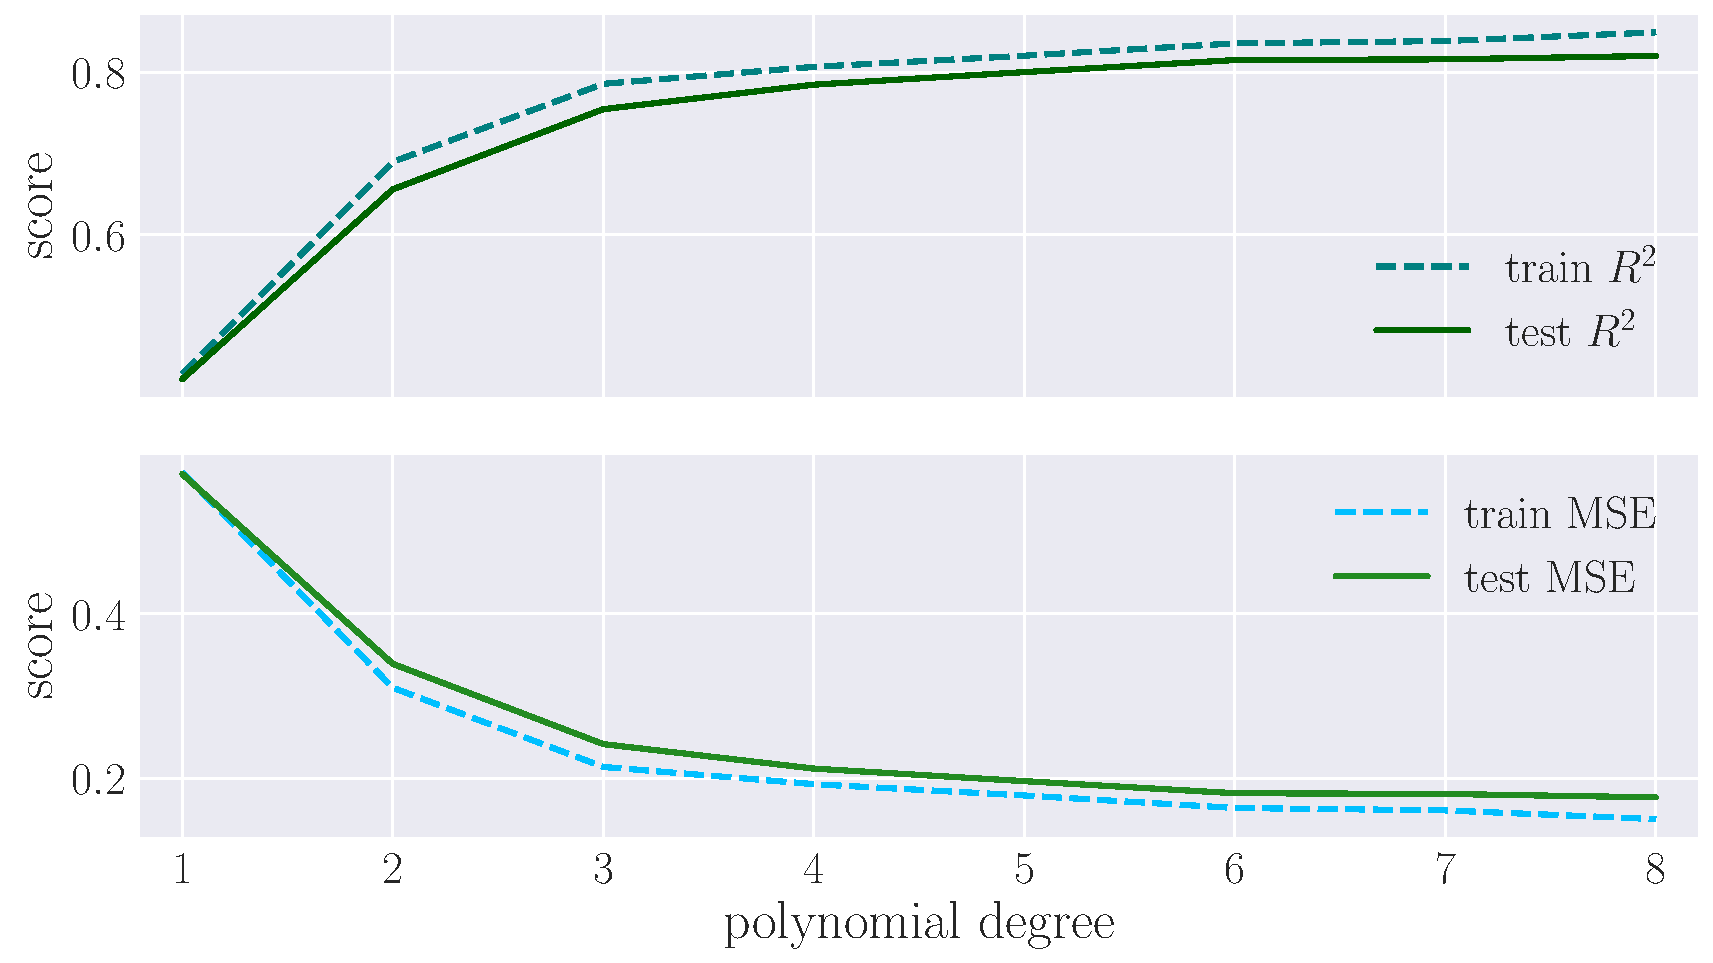
\includegraphics[width=\linewidth]{Franke/MSE_R2_scores_ols.pdf}
                \caption{MSE and $R^2$ scores for train and test data for polynomials up to order $d=5$ for the OLS analysis of the Franke function ($N=20$, $\eta=0.1$). We  see that for the polynomial degrees present, the MSE decrease, while the $R^2$-score increase towards 1 for increasing polynomial  degree. }
                \label{fig:mse_and_r2_for_order5}
            \end{figure}
            
            
            We want to investigate the effect of the noise parameter $\eta$ on the MSE for our model. In \Fig{mse_for_different_noise_ols} we have plotted this for $\eta = 10^{\gamma}, \gamma\in\{-4,-3,-2,-1,0\}$. We observe that for large noise ($\eta=1$) the MSE is high, which is expected. For lower noise the MSE is lower (pay attention to the logarithmic scale for the MSE). The MSE also decreases with polynomial degree for low noise, emphasising what we found in \Fig{mse_and_r2_for_order5}. In order to represent something slightly more physical than a smooth curve (e.g. terrain data), we will use $\eta=0.1$ for our further analysis. 

            \begin{figure}
                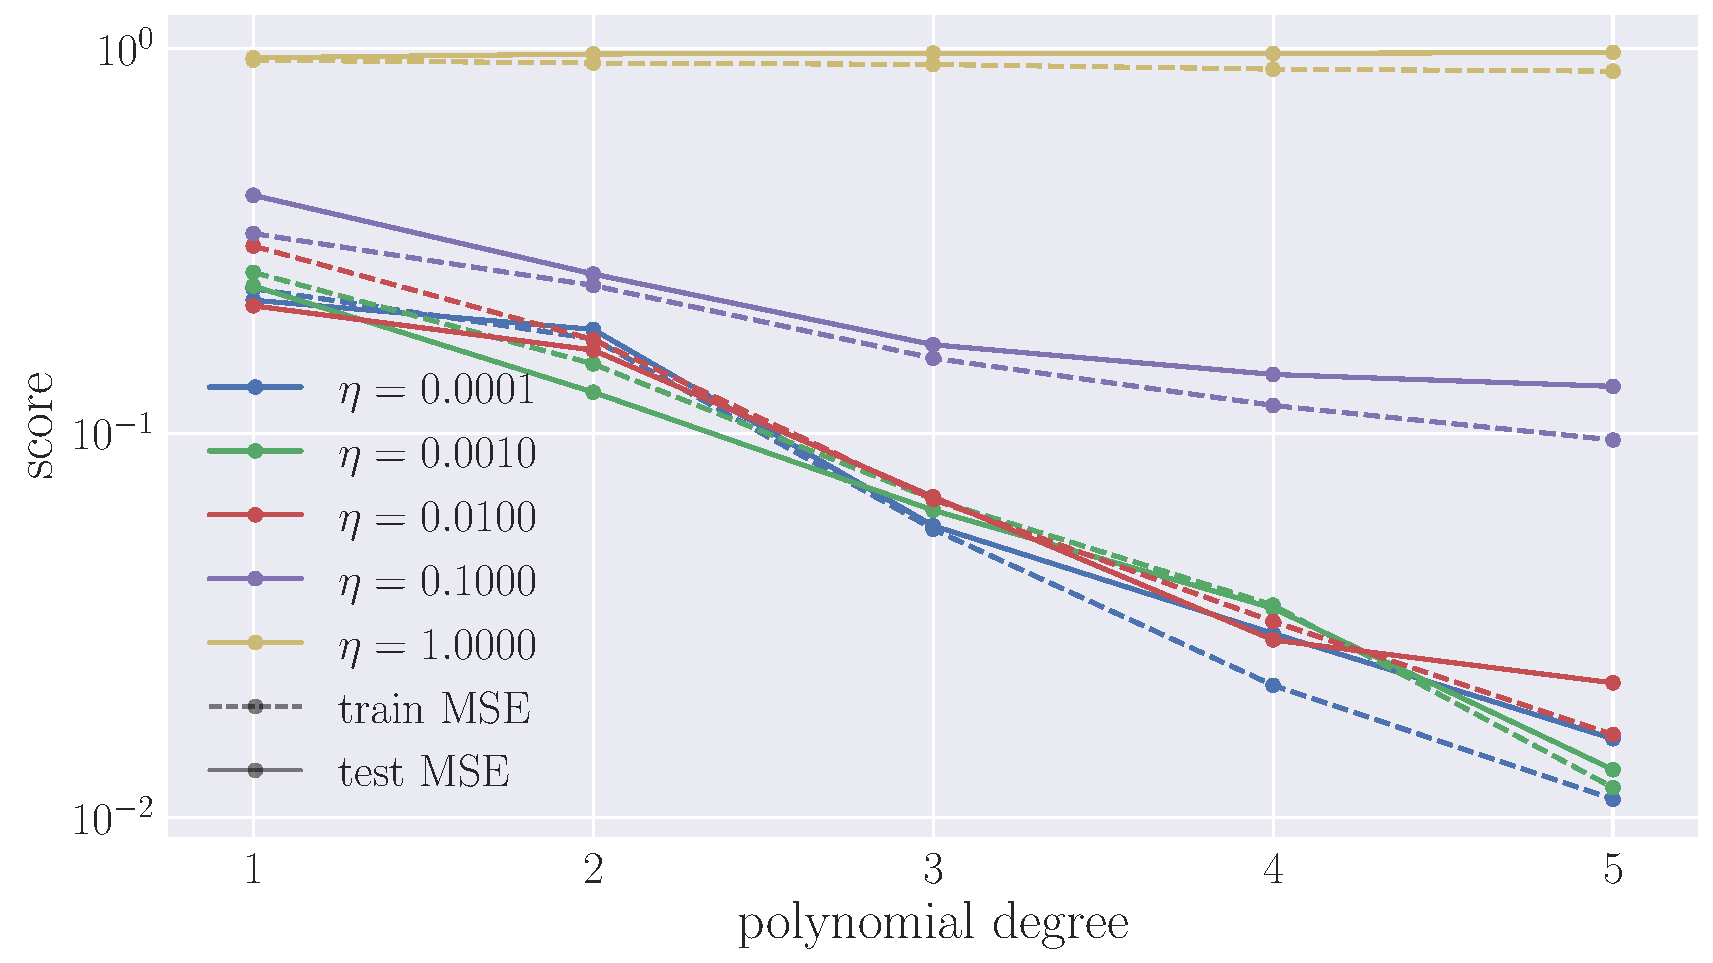
\includegraphics[width=\linewidth]{Franke/error_vs_noise_ols.pdf}
                \caption{MSE for train and test data for polynomials up to order $d=5$ for the OLS analysis of the Franke function ($N=20$), for different noise parameters $\eta = 10^{\gamma}, \gamma\in\{-4,-3,-2,-1,0\}$. The MSE is large for noisy function (large $\eta$), but decreasing with polynomial degree.}
                \label{fig:mse_for_different_noise_ols}
            \end{figure}


            From \Fig{mse_and_r2_for_order5} we got the impression the higher the polynomial degree, the better the model. We want to investigate this further and look at how the training and generalisation errors behave for polynomials of order up to 20. The model is trained on the training data, but the MSE is evaluated for both the training and test data. The result is shown in \Fig{model_complexity_ols}. The MSE of the training data decrease as the polynomial degree increase. This is not a surprise, since the model will traverse more points of the training data exactly as the complexity ($d$) increase. The MSE of the test data however, seem to decrease at first, but then rapidly increase as the polynomial degree increase. This is similarly explained with the model being too tailored to the training data. When applied to the test data (which consist of completely different pieces of data), the model fails to make accurate predictions. This is an indicator of a phenomenon called \textit{over-fitting}: when the model is so tailored to the training data it is unable to make accurate predictions on other, similar data. For a more reliable result, the data in \Fig{model_complexity_ols} is generated by bootstrapping the training data with $k=400$ as explained in \Sec{bootstrap}. We consider 400 a suitable number of bootstraps in order to gain an accurate result without requiring too much computational time. Without showing it here, a larger number of bootstraps yield more or less the same results.

            \begin{figure}
                \includegraphics[width=\linewidth]{Franke/MSE_ols_BS.pdf}
                \caption{MSE for train and test data for polynomials up to order $d=12$ for the OLS analysis of the Franke function ($N=20$, $\eta=0.1$) generated with a $k=400$ bootstrap. When we increase the model complexity  up to order $d=12$ we easily  spot that the MSE for train data starts to diverge, which could be a sign of over-fitting.}
                \label{fig:model_complexity_ols}
            \end{figure}

            We take the analysis further and consider the bias-variance tradeoff, as explained in \Sec{bias_variance_tradeoff}. The result is shown in \Fig{bias_variance_ols} where we clearly see that for low-order polynomials the error occurs mostly from bias, but from variance for high-order polynomials. There is a tradeoff, where the total error switches main dependence from bias to variance, ultimately minimising it. In \Fig{bias_variance_ols} this  tradeoff can be found around polynomial degree $d\approx 5$.

            
            \begin{figure}
                \includegraphics[width=\linewidth]{Franke/tradeoff_ols.pdf}
                \caption{Bias, variance and residual error for polynomials up to order $d=12$ for the OLS analysis of the Franke function ($N=20$, $\eta=0.1$), generated with a $k=400$ bootstrap. We see that for low polynomial degrees there is a high bias and low variance, the opposite for larger degrees, and we find a trade off at around $d\approx 5$.}
                \label{fig:bias_variance_ols}
            \end{figure}
            
            
            A similar reasoning can be made by applying cross-validation as a resampling technique, as explained in \Sec{k_fold}. The result of this is shown in \Fig{cross-validation_ols} where we have used $k$-fold cross-validation for $k=5,6,\dots,10$ of the training data and found the corresponding MSE for the training and "test" data. From the graph we see that MSE for the training data decrease with polynomial degree, which is expected w.r.t. to previous discussion. Similarly the MSE for the test data reaches a minimum and seem to diverge. The minimum point is found at $d\approx 5$.

            \begin{figure}
                \includegraphics[width=\linewidth]{Franke/MSE_ols_CV.pdf}
                \caption{CV accuracy for polynomials up to order $d=12$ for the OLS analysis of the Franke function ($N=20$, $\eta=0.1$) generated with an $k\in[5,10]$-fold cross validation. We observe a similar behaviour with \Fig{model_complexity_ols} where the MSE for the test data reaches a minimum at $d=5$ and then seem to diverge. }
                \label{fig:cross-validation_ols}
            \end{figure} 
            
            It has become apparent that the polynomial degree that seem to fit our data the best is $d=5$, and so we want to investigate this model further. Considering the bootstrapping resampling technique we make a histogram of the average MSE with samples from each iteration for $d=5$. The  result is shown in \Fig{mse_hist_ols}. We may interpret these histograms (if they were to be normalised) as a probability distribution, where the expectation value of the MSE for the train and test data is the MSE which corresponds to the highest probability. As discussed in section \Sec{bootstrap}, if $k\to\infty$ then this probability distribution approaches the normal distribution and the expectation value would be the mean. Translating this to the specific case at hand here, the most likely MSE value can interpreted as the MSE value with the highest frequency for both the train and test data. If we compare this plot to \Fig{model_complexity_ols} we see that the numerical values of MSEs coincide, with the test MSE being slightly higher than the test MSE. 

            \begin{figure}
                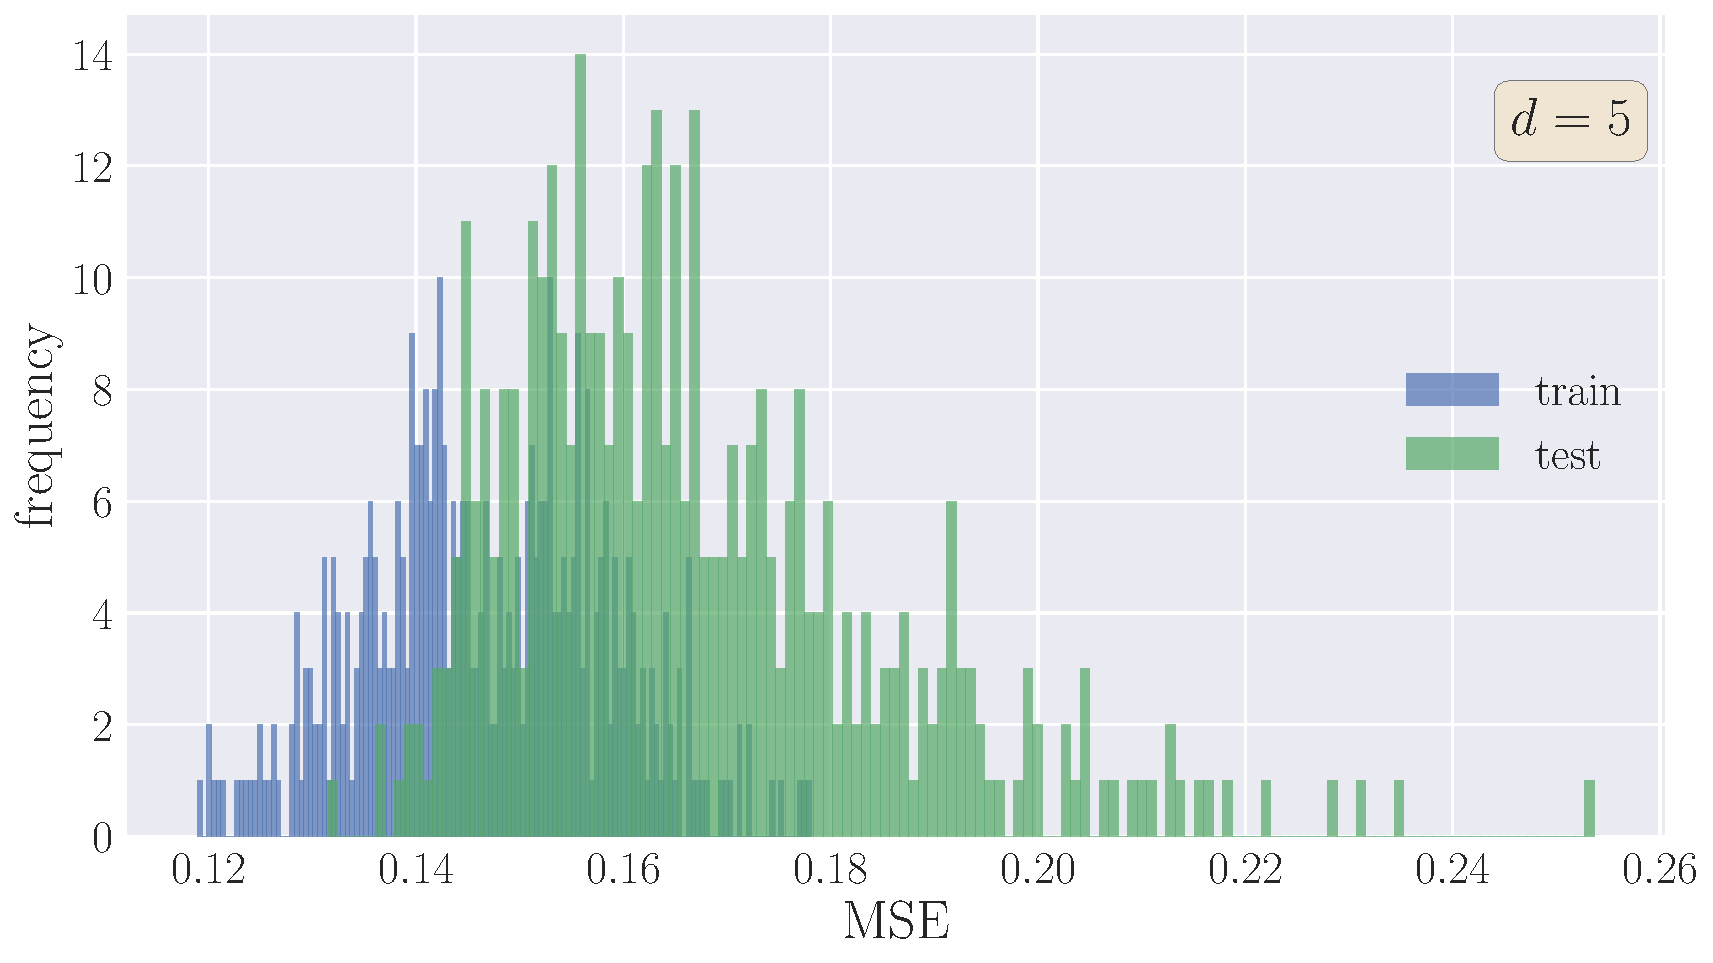
\includegraphics[width=\linewidth]{Franke/MSE_hist_OLS.pdf}
                \caption{Histogram of average MSE for train and test data for polynomial degree $d=5$ for the OLS analysis of the Franke function ($N=20$, $\eta=0.1$), generated with a $k=400$ bootstrap. The train data seem to have a slightly lower MSE than the test data. This is consistent with \Fig{model_complexity_ols} for $d=5$.}
                \label{fig:mse_hist_ols}
            \end{figure}

            We also investigate how the mean of the feature parameters $\svec{\beta}$ behave while bootstrapping for $d=5$. Since both the design matrix $X$ and the data $\vec{y}$ are scaled to have mean $\mu=0$, we also expect the mean of the feature parameters to be centred around 0, as emphasised in \Fig{beta_with_standard_deviation} where 0 appear to be the by-eye mean.  The resulting histogram is shown in figure \Fig{beta_hist_ols}, where we see a frequency distribution centred at around 0, as expected. 

            \begin{figure}
                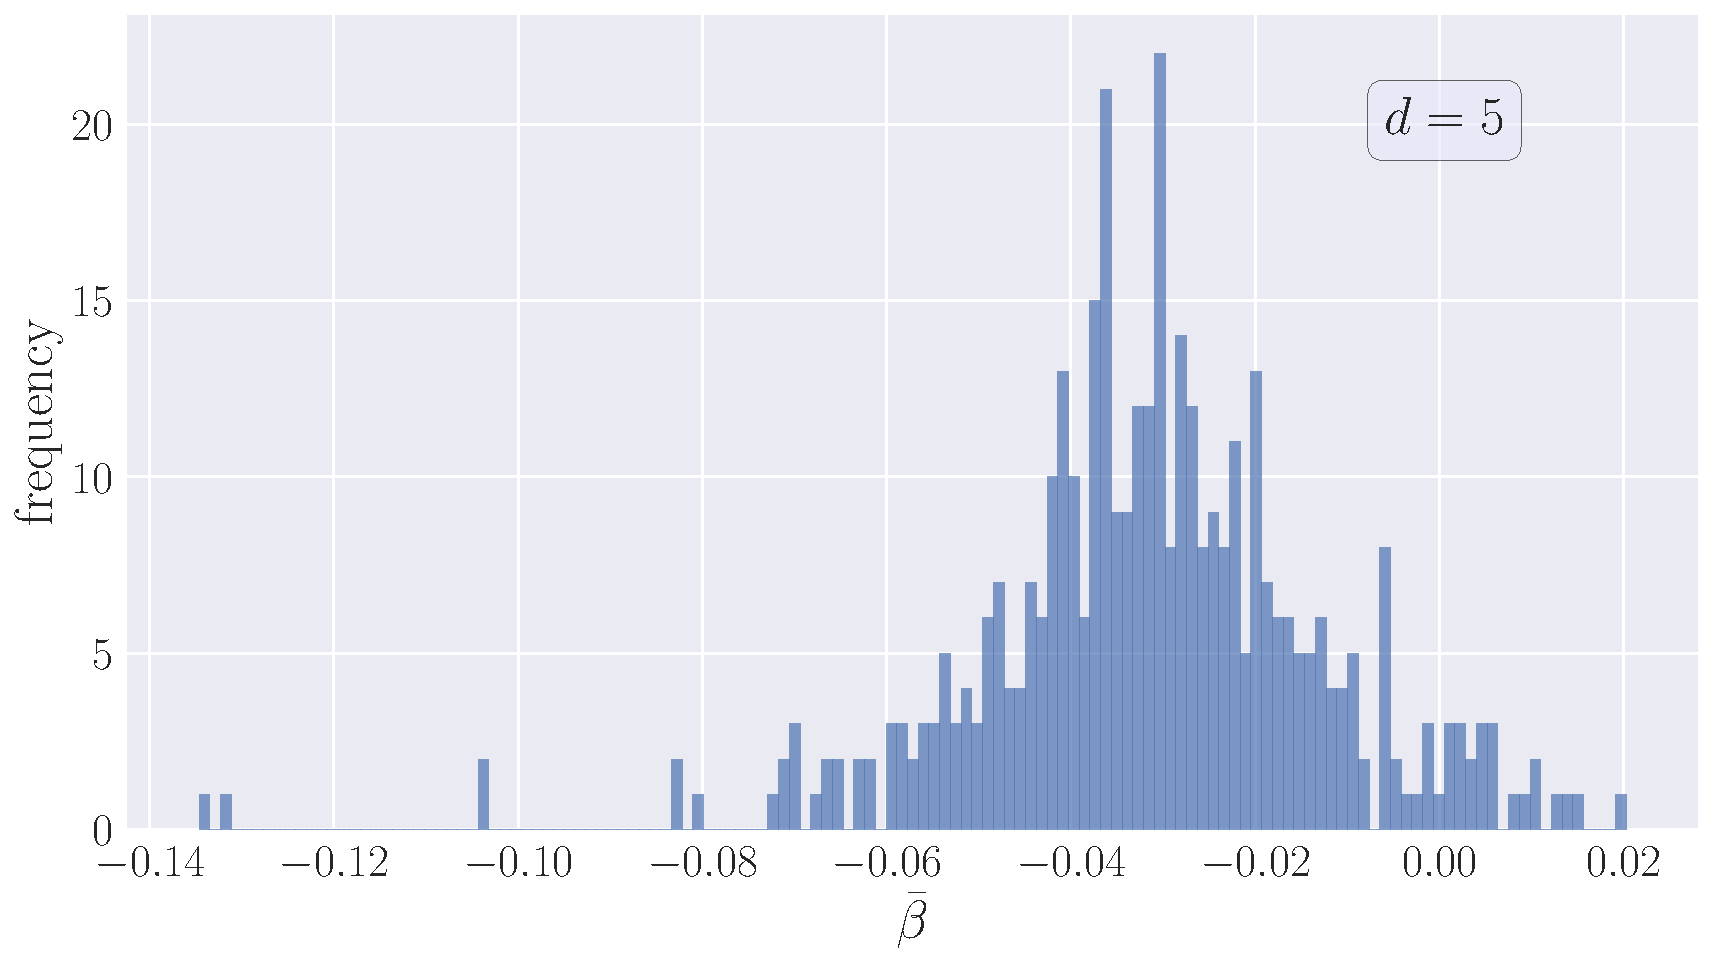
\includegraphics[width=\linewidth]{Franke/beta_hist_OLS.pdf}
                \caption{Histogram of average feature parameters $\svec{\beta}$ for polynomial degree $d=5$ for the OLS analysis of the Franke function ($N=20$, $\eta=0.1$), generated with a $k=400$ bootstrap. Since all the features are scaled to mean $\mu=0$, we expect the average features parameter to be close to 0, which is consistent both with this histogram, but also with \Fig{beta_with_standard_deviation} for $d=5$. }
                \label{fig:beta_hist_ols}
            \end{figure}
            


        

        \subsubsection{Ridge}\label{sec:rigdeanalysis}

        We continue our analysis of the model using $d=5$, but now for Ridge regression, where the free parameter will be the penalty parameter $\lambda$. The technicalities of this method is explained in section \Sec{Ridge}. A natural place to start this analysis is to see how the MSE change for different penalty parameters $\lambda$, and we to this by using the two resampling techniques previously discussed. In \Fig{cross-validation_ridge} we see how the MSE for both the train and the test data change as a function of $\lambda$. This plot was generated using an 8-fold cross-validation. Since $\lambda=0$ corresponds to OLS analysis, we would expect the MSEs for low $\lambda$ to be fairly similar to the OLS values. If we compare this with \Fig{model_complexity_ols} and \Fig{cross-validation_ols} we see that this is indeed the case when $d=5$. We also observe that both the test and train MSEs increase when we increase $\lambda$. 

        \begin{figure}
            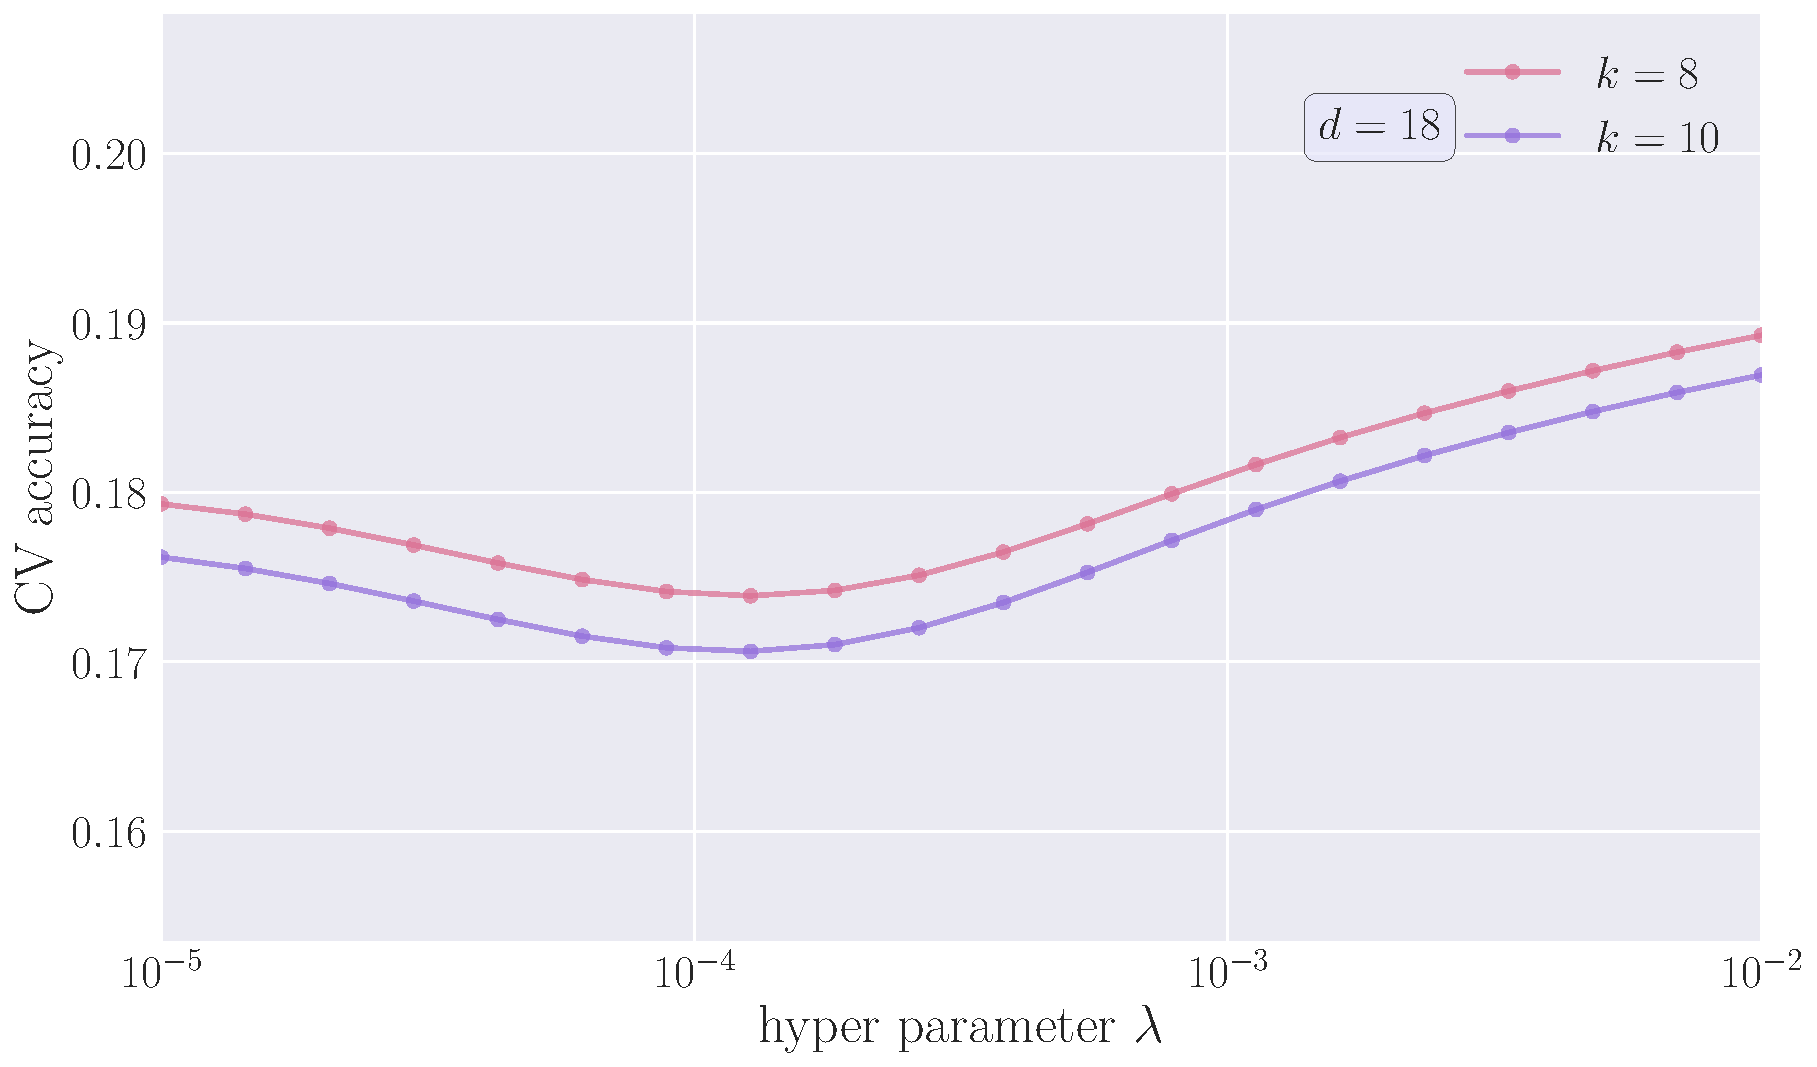
\includegraphics[width=\linewidth]{Franke/MSE_ridge_CV.pdf}
            \caption{CV accuracy for polynomial of degree $d=5$, as function of the penalty parameter $\lambda$ for the ridge analysis of the Franke function ($N=20, \eta=0.1$) generated with both a 6-fold, 8-fold and 10-fold cross validation.}
            \label{fig:cross-validation_ridge}
        \end{figure}

        However, when we repeat the analysis but generate the plot using a $k=400$ bootstrap instead, as shown in \Fig{bootstrapping_ridge}, we see that the test MSE decrease to a minimum and remain low when we increase $\lambda$. We also note that the $\lambda$ which minimised the test MSE is found numerically to be $\lambda^\mathrm{Ridge} = 7.85\cdot10^{-5}$ given to two significant figures. 


        \begin{figure}
            \includegraphics[width=\linewidth]{Franke/MSE_ridge_BS.pdf}
            \caption{MSE for train and test data for polynomial of degree $d=5$, as a function of the penalty parameter $\lambda$ for the ridge analysis of the Franke function ($N=20, \eta=0.1$) generated using a $k=400$ bootstrap. }
            \label{fig:bootstrapping_ridge}
        \end{figure}

        We perform the bias-variance decomposition with a $k=400$ bootstrap which results in the plot shown in \Fig{bias_variance_ridge}. We see that the variance remains low for this $\lambda$ range, while the residual error follows the bias closely. They both seem to reach a minimum at around $\lambda\approx 10^{-4}$ which coincides very well with $\lambda^\mathrm{Ridge}$. This is expected since Ridge regression is a biased model. 

        \begin{figure}
            \includegraphics[width=\linewidth]{Franke/tradeoff_ridge.pdf}
            \caption{Bias, variance and residual error for polynomial of degree $d=5$, as a function of the penalty parameter $\lambda$ for the ridge analysis of the Franke function ($N=20, \eta=0.1$) generated with a $k=400$ bootstrap. We see that the variance remain low, and the bias and error terms follow each other.}
            \label{fig:bias_variance_ridge}
        \end{figure}

        We investigate the model further by using $\lambda^\mathrm{Ridge}$ and plot the frequencies of the average MSE for the train and test data as a histogram using a $k=400$ bootstrap, shown in \Fig{mse_hist_ridge}. From this we see that the test MSE is slightly lower that the train MSE which is in accordance with \Fig{bootstrapping_ridge}.

        \begin{figure}
            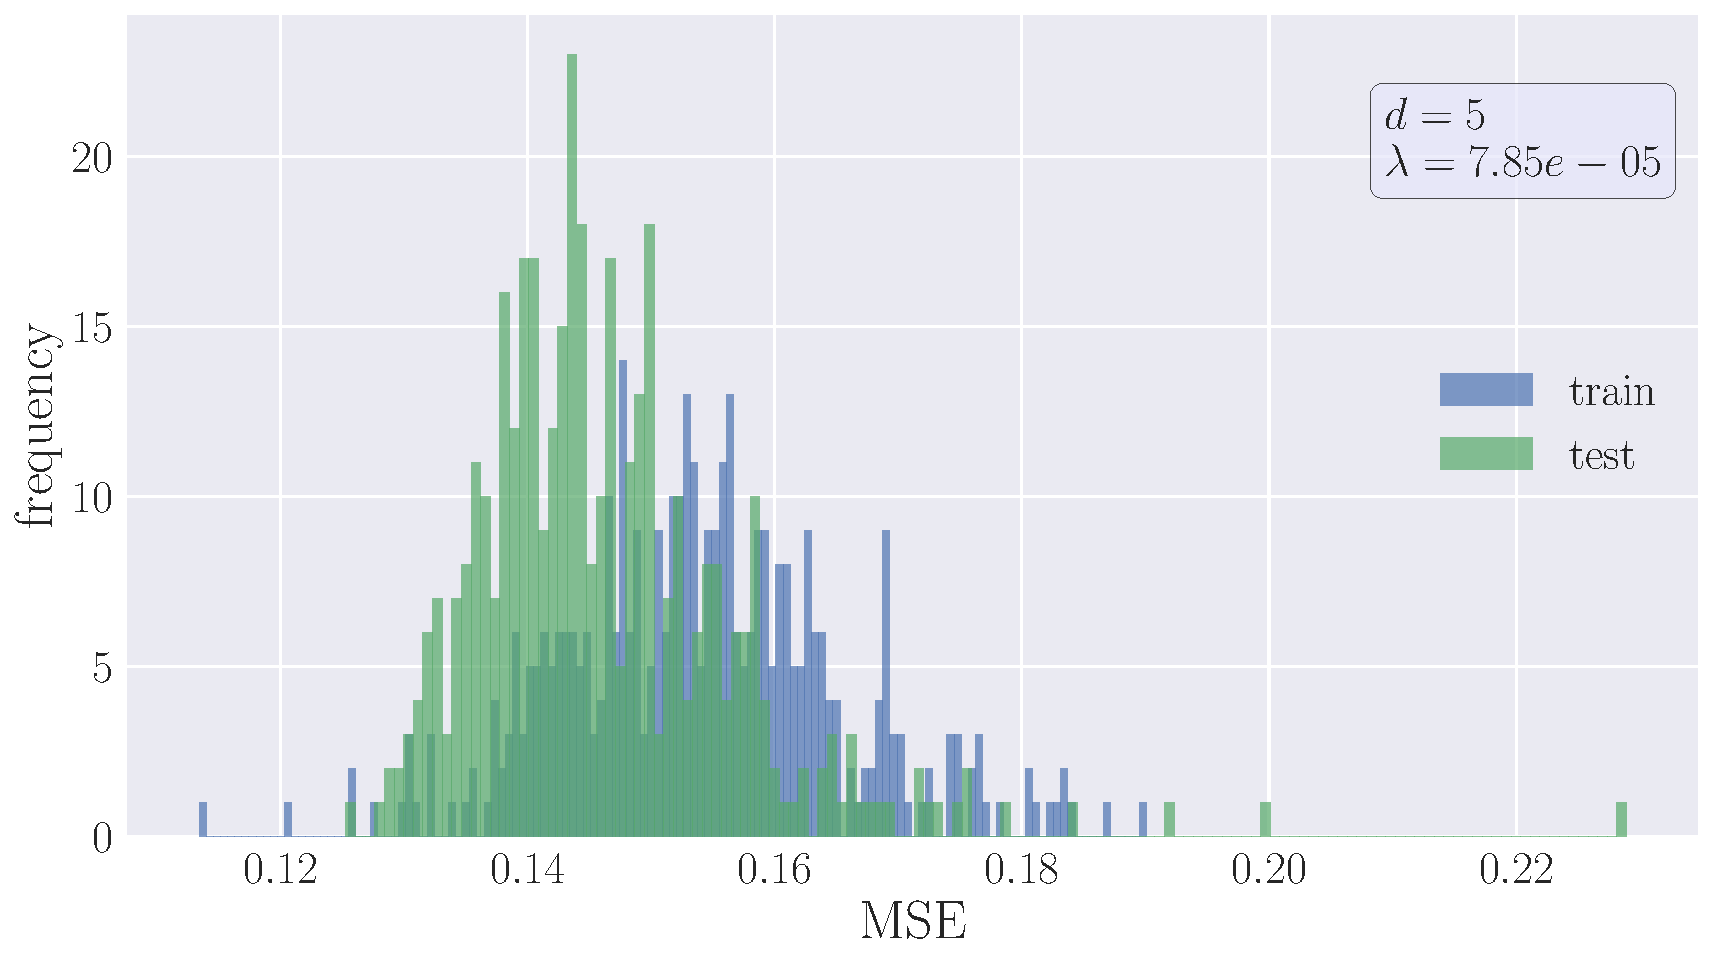
\includegraphics[width=\linewidth]{Franke/MSE_hist_ridge.pdf}
            \caption{Histogram of average MSE for train and test data for polynomial degree $d=5$ for the ridge analysis of the Franke function ($N=20$, $\eta=0.1$), generated with a $k=400$ bootstrap and $\lambda=7.85\cdot 10^{-5}$. The test data has a lower MSE than the train data. This is consistent with \Fig{bootstrapping_ridge} for this value of $\lambda$.}
            \label{fig:mse_hist_ridge}
        \end{figure}

        We may also plot the histogram of the average of the feature parameters $\svec{\beta}$. We would perhaps guess that these values should be centered around 0, using similar arguments as for \Fig{beta_hist_ols}. However, the penalty parameters $\lambda$ will shrink $\svec{\beta}$-values corresponding to small singular values in the design matrix $X$. It therefore gives emphasise to the $\svec{\beta}$-values corresponding to large singular values of the design matrix. This may explain the skew towards negative parameter values which we observe in \Fig{beta_hist_ridge} where we plot the abovementioned histogram. 
        \begin{figure}
            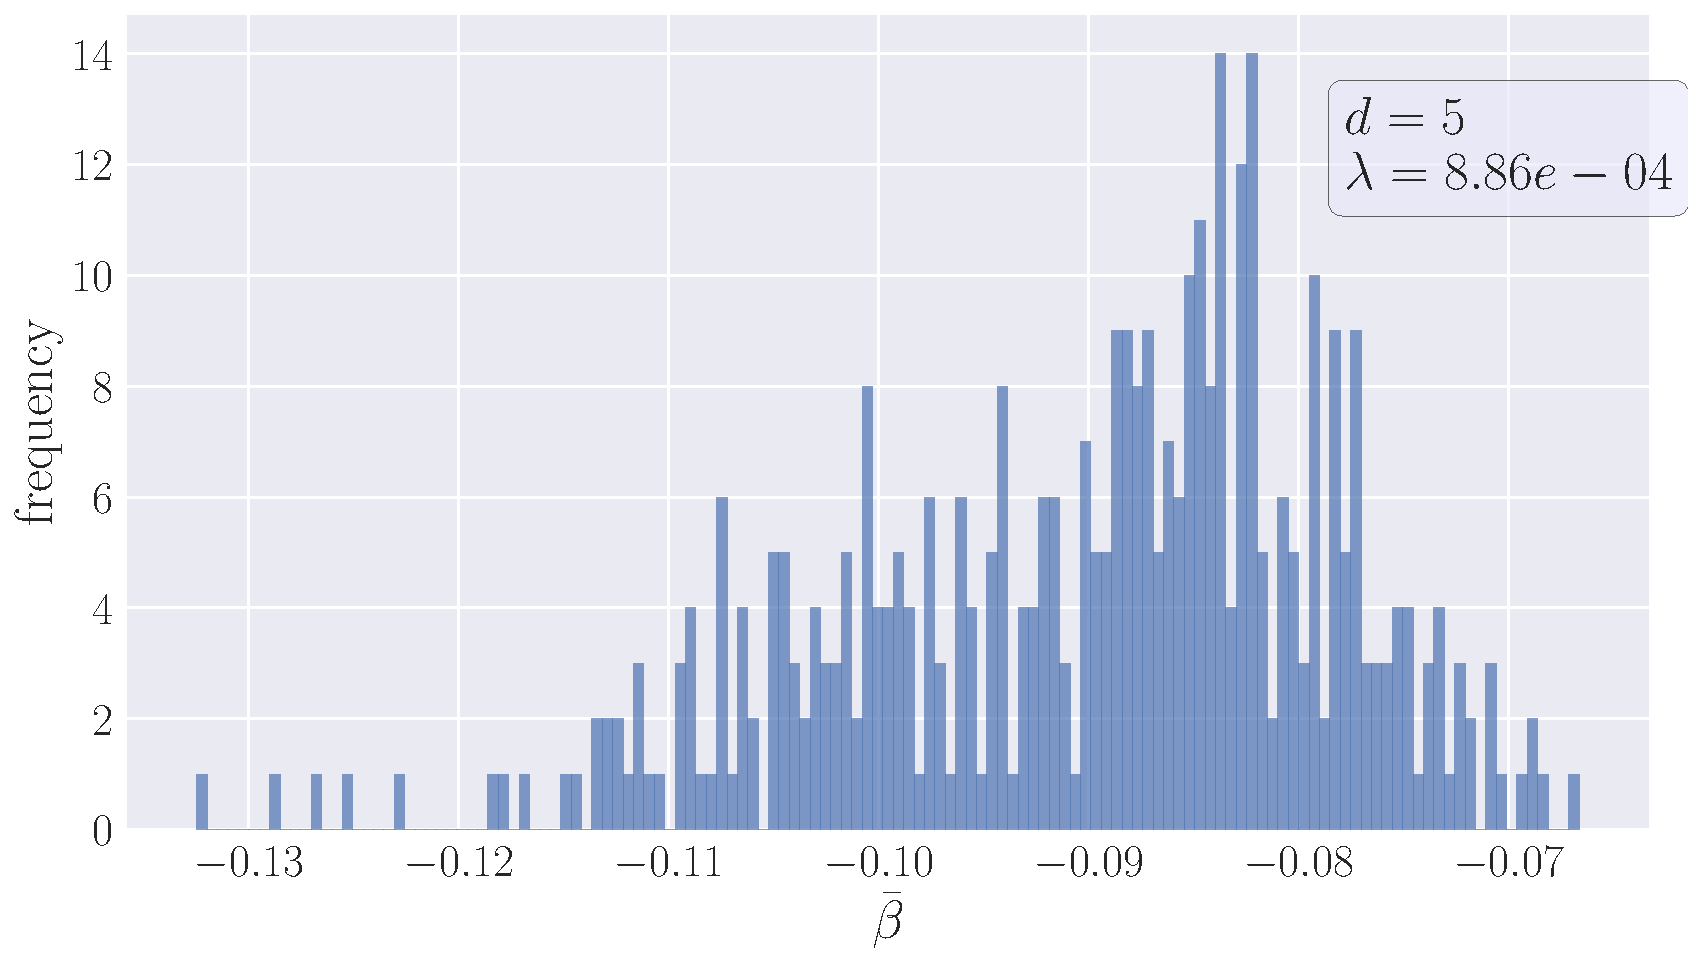
\includegraphics[width=\linewidth]{Franke/beta_hist_ridge.pdf} 
            \caption{Histogram of average feature parameters $\svec{\beta}$ for polynomial degree $d=5$ for the ridge analysis of the Franke function ($N=20$, $\eta=0.1$), generated with a $k=400$ bootstrap and $\lambda=7.85\cdot 10^{-5}$. With the same reasoning as in \Fig{beta_hist_ols} we would expect these to be centred around 0. However, the penalty parameter shrinks certain beta values, which may explain the skew observed here.}
            \label{fig:beta_hist_ridge}
        \end{figure}











        \subsubsection{Lasso}\label{sec:lassoanalysis}

        We now make a similar analysis, but we use the Lasso regression analysis instead, with a slightly different approach. Instead of looking for the optimal penalty parameter $\lambda$ for a given polynomial degree $d$, we seek to find them at them simultaneously, by performing a grid search on a grid of MSE values, which are functions of both $\lambda$ and $d$. The result is shown in \Fig{gridsearch_cv_lasso}, where we perform an 8-fold cross-validation and present the resulting MSE as a heatmap. 
        What we draw from this heatmap is that the there seems to be an optimal band across polynomial degrees for the penalty parameter $\lambda =2.15\cdot10^{-5}$. Our grid search yields the border value of the polynomial degree ($d=14$) which could indicate that the true best fit is of a higher polynomial degree. However, due to the fact that a polynomial of degree $d=14$ is high for a $N=20$ grid, and it becomes very computationally expensive to run the Lasso analysis on such models, we restrict ourselves to not go beyond this. On the other hand, higher polynomial degrees seem plausible with the Lasso regression scheme, as the penalty parameter is able to drive unimportant features to zero, reducing the dimensionality of the model. We thus take a closer look at the results of such a model ($d=14$). 

        \begin{figure}
            \includegraphics[width=\linewidth]{Franke/MSE_heatmap_lasso_CV.pdf}
            \caption{Heatmap of the prediction MSE as function of both polynomial degree $d\in[6,14]$ and penalty parameter $\lambda$ for the Lasso analysis of the Franke function ($N=20, \eta=0.1$), generated with an 8-fold cross validation.}
            \label{fig:gridsearch_cv_lasso}
        \end{figure}

        \Fig{cross-validation_lasso} shows the MSE for the test data predictions for two different cross-validations: 6-fold and 8-fold. This plot confirms that there is an optimal value for $\lambda\in[10^{-5}, 10^{-4}]$ that minimise the MSE, and we have reason to believe it is the same $\lambda$ that we found in \Fig{gridsearch_cv_lasso}.

        \begin{figure} 
            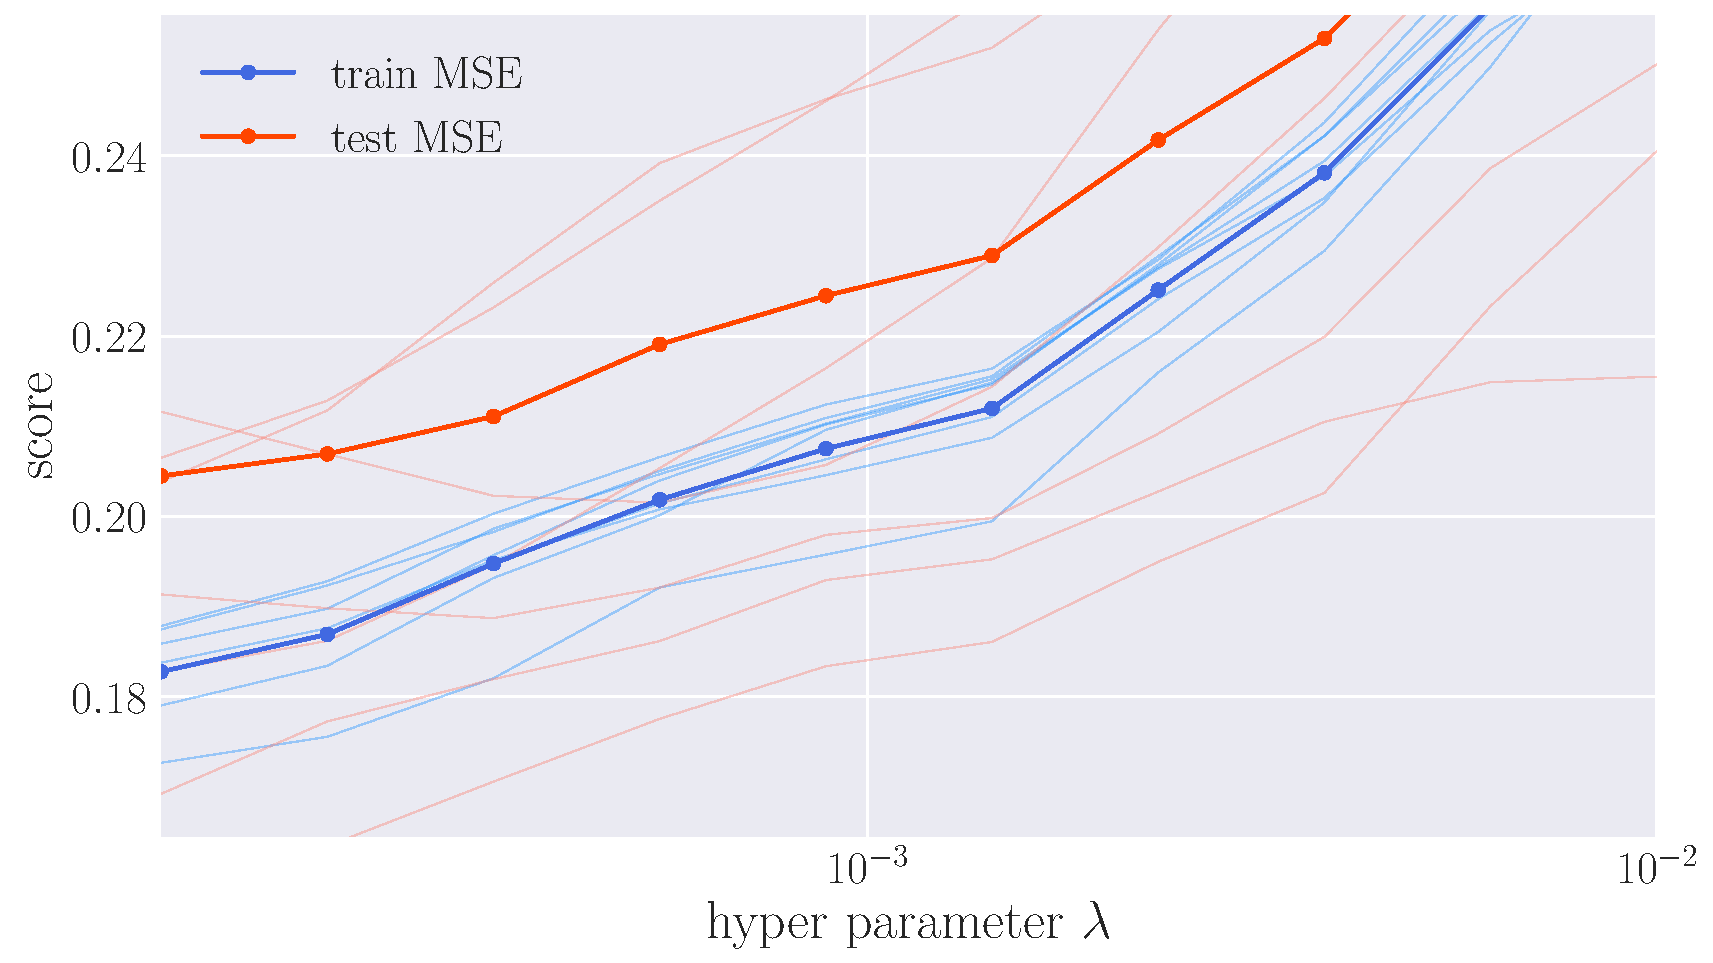
\includegraphics[width=\linewidth]{Franke/MSE_lasso_CV.pdf}
            \caption{CV accuracy for polynomial of degree $d=14$, as function of the penalty parameter $\lambda$ for the Lasso analysis of the Franke function ($N=20, \eta=0.1$) generated with both a 6-fold and 8-fold cross validation.}
            \label{fig:cross-validation_lasso}
        \end{figure}


        If we then consider the MSE found by a $k=40$ bootstrap as seen in \Fig{bootstrapping_lasso} for larger $\lambda$ we see that there is perhaps a more optimal $\lambda$ around $10^{-3}$ which yield a lower MSE of $\approx 0.15$. 

        \begin{figure}
            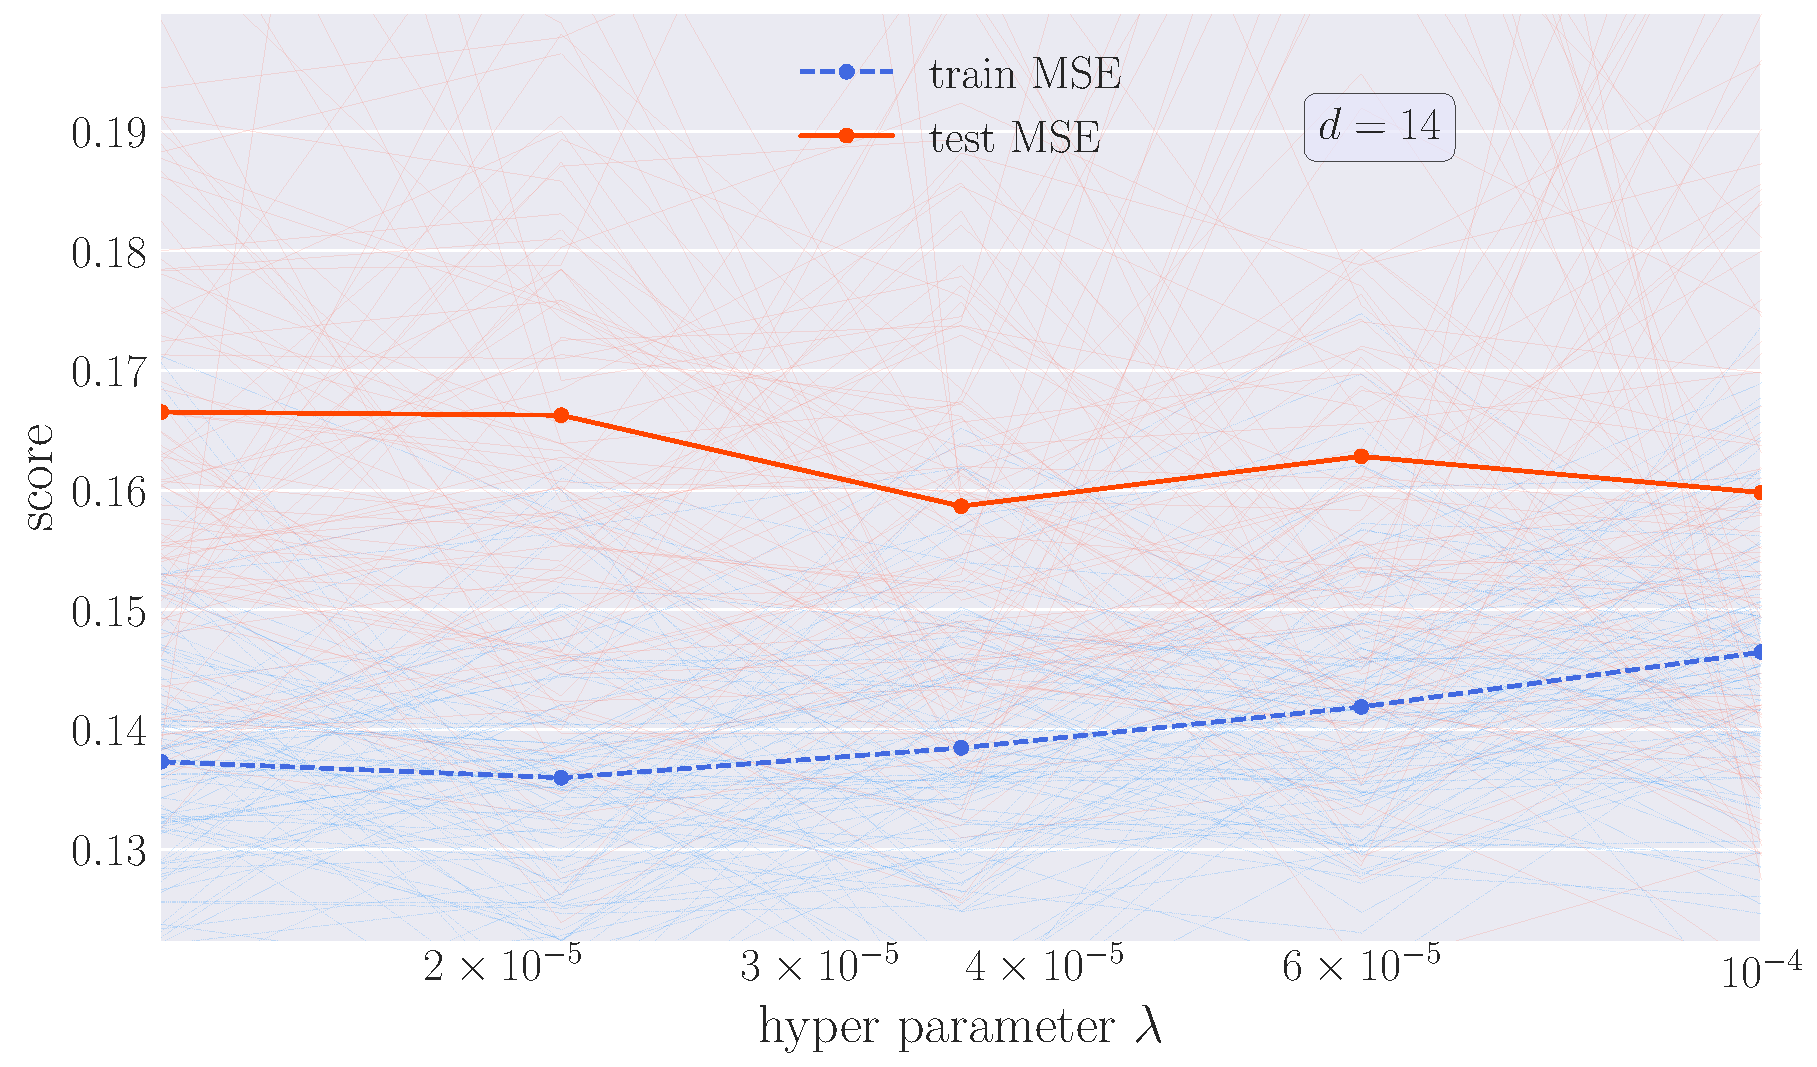
\includegraphics[width=\linewidth]{Franke/MSE_lasso_BS.pdf}
            \caption{MSE for train and test data for polynomials of degree $d=14$, as a function of the penalty parameter $\lambda$ for the Lasso analysis of the Franke function ($N=20, \eta=0.1$) generated using a $k=40$ bootstrap. }
            \label{fig:bootstrapping_lasso}
        \end{figure}


        \Fig{bias_variance_lasso} show the bias variance trade off for the Lasso regression for $d=14$ made with the same $k=40$ bootstrap, for computational efficiency. We draw from this that the Lasso regression scheme has a low variance, but high bias for the $\lambda$ values considered, with perhaps the same optimal $\lambda$ at around $10^{-3}$.


        \begin{figure}
            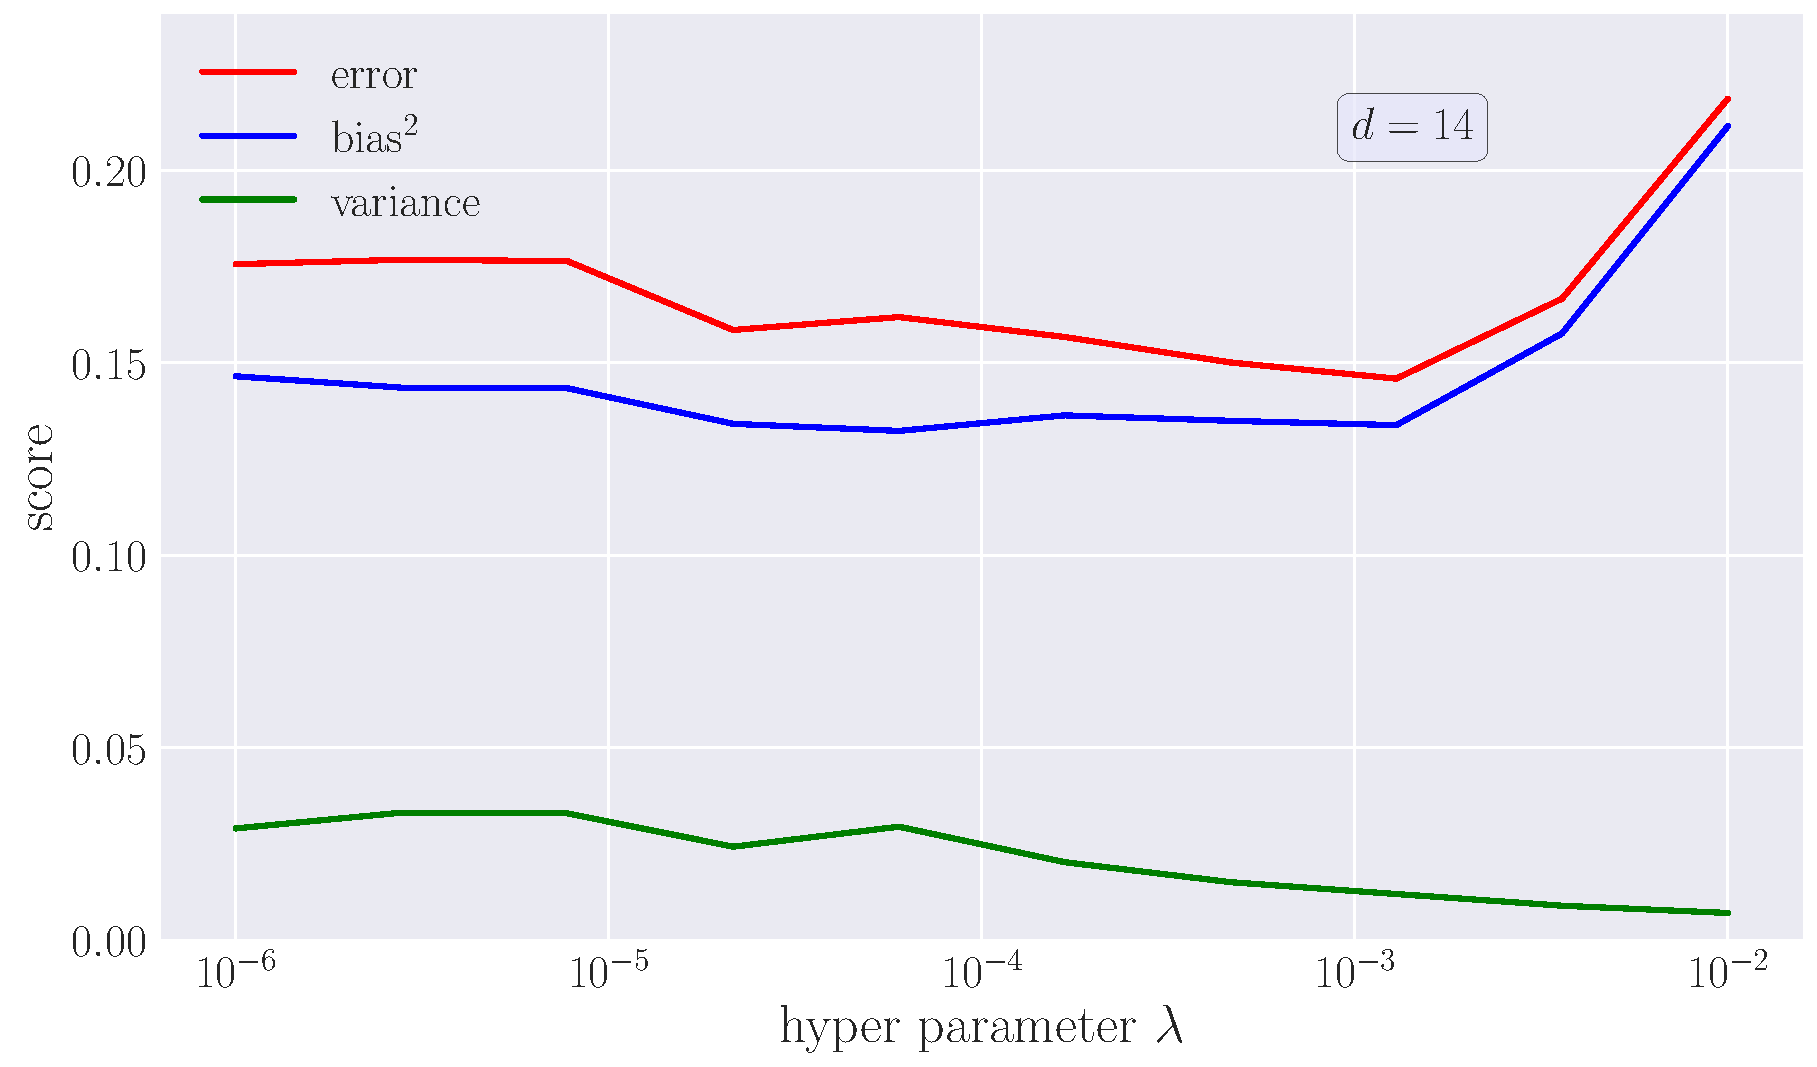
\includegraphics[width=\linewidth]{Franke/tradeoff_lasso.pdf}
            \caption{Bias, variance and residual error for polynomial of degree $d=14$, as a function of the penalty parameter $\lambda$ for the Lasso analysis of the Franke function ($N=20, \eta=0.1$) generated with a $k=40$ bootstrap.}
            \label{fig:bias_variance_lasso}
        \end{figure} 
        

    \subsection{Regression analysis for real terrain data}\label{sec:reganalysis_real_data}

    By the courtesy of \citep{EarthExplorer}, we were able to extract the terrain data of a part of the Crand Ganyon in Arizona, United States. To properly retrieve the geographical coordinates of the map is somewhat circumstantial and utterly unimportant to this task, we to not mind these in this project. We read the GeoTIFF and choose an area from which we extract a coarse grid. In particular, the original cutout area in question consists of $N=900$ points in the $x$ and $y$ direction each. In order to speed up our codes, we use only the data from every \nth{30} $x$- and $y$-point, leaving us with $N=30$ in each direction. We now have $N^2=900$ $z$-points representing relative altitude, of which 20\% are saved for verification. After splitting randomly, we scale the data using the z-score normalisation explained in \Sec{scaling}. It would not make sense to concern ourselves with the vertical units (the actual altitude), as we already have omitted the horizontal units. The scaled data is what we aspire to work with and is presented in its completeness in \Fig{gc_data}.

    \begin{figure}
        \includegraphics[width=\linewidth]{terrain/data3D.pdf}
        \caption{Scaled terrain data representing a part of the Grand Canyon. Data points are extracted to fit a $N=30$ grid. This data is scaled according to the discussion in \Sec{scaling}, so numerical data point values are of no interest to us and thus omitted in the plot.}
        \label{fig:gc_data}
    \end{figure}

    Moving forward, we essentially repeat the analysis in \Sec{reganalysis_franke} for the terrain data. Starting with the OLS method, we expect the need of a higher order polynomial than for the Franke funtion.

        \subsubsection{OLS}\label{sec:gc_olsanalysis}

        We perform the least squares fitting as elaborated in \Sec{OLS} on the training data for polynomials of order $d=1,2,..., 20$. For $d\leq 7$, the resulting $\optbeta^\text{OLS}$ is plotted in \Fig{gc_beta_with_standard_deviation}, where we have grouped the parameters such that $\beta^{(d_i)}$ is the mean of the elements belonging to the same order $d_i$, i.e. $\beta^{(1)} = \nicefrac{1}{2}(\beta_1 + \beta_2)$, $\beta^{(2)} = \nicefrac{1}{3}(\beta_3 + \beta_4 + \beta_5)$, etc. 

        \begin{figure}
            \includegraphics[width=\linewidth]{terrain/beta_ols.pdf}
            \caption{Numerical value of the mean of the feature parameters $\beta$ for each polynomial degree, with 1$\sigma$ error bars, for polynomials up to order $d=7$ for the OLS analysis of the terrain data. We note that the parameters for similar features tend to have the same sign across models, however there is an increase in parameter magnitude.}
            \label{fig:gc_beta_with_standard_deviation}
        \end{figure}

        
        \begin{figure}
            \includegraphics[width=\linewidth]{terrain/MSE_ols_CV.pdf}
            \caption{CV accuracy for for polynomials up to degree $d=20$, for the OLS analysis of the terrain data, generated with both a 6-fold, 8-fold and 10-fold cross validation. Common for all is that the CV accuracy is best at around $d=6$.}
            \label{fig:gc_cv_errors_ols}
        \end{figure}

        After performing a simple $k$-fold cross-validation to optimise the model, we see from \Fig{gc_cv_errors_ols} that it clearly prefers order $d=6$. We continue with the bootstrap resampling technique to verify that this complexity is preferable for our test data as well. In \Fig{gc_model_complexity_ols} we see the expected behaviour of the training and prediction error per increasing model complexity.
        

        \begin{figure}
            \includegraphics[width=\linewidth]{terrain/MSE_ols_BS.pdf}
            \caption{MSE for train and test data for polynomials up to degree $d=20$ for the OLS analysis of the terrain data, generated with a $k=400$ bootstrap. We deduce from the plot that test MSE is minimised at around $d=6$}
            \label{fig:gc_model_complexity_ols}
        \end{figure}

        The choice $d=6$ still seems sensible, but let us decompose the bootstrap prediction error into bias and variance as in section \Sec{bias_variance_tradeoff}. The plot in \Fig{gc_bias_variance_ols} points to a conclusion that OLS-estimations with $d\geq 7$ is over-fitting the data. However, that might not be the case if we are able to penalise the $\beta_j$'s. We move on to the penalised estimation models.

        \begin{figure}
            \includegraphics[width=\linewidth]{terrain/tradeoff_ols.pdf}
            \caption{Bias variance and residual error for polynomials up to degree $d=20$ for the OLS analysis of the terrain data, generated with a $k=400$ bootstrap. The best bias variance trade off appear to be at around $d=6$.}
            \label{fig:gc_bias_variance_ols}
        \end{figure}


        \subsubsection{Ridge}\label{sec:gc_ridgeanalysis}

        % something about lower limig lambda?

        The search for an optimal model begins with a grid search where we limit ourselves to $d\in[4, 20]$ and $\lambda=10^{-\gamma}, 5 \geq \gamma \geq 2$. The grid search is somewhat computationally expensive, at least for large $d$ and small $\lambda$.
        
        \begin{figure}
            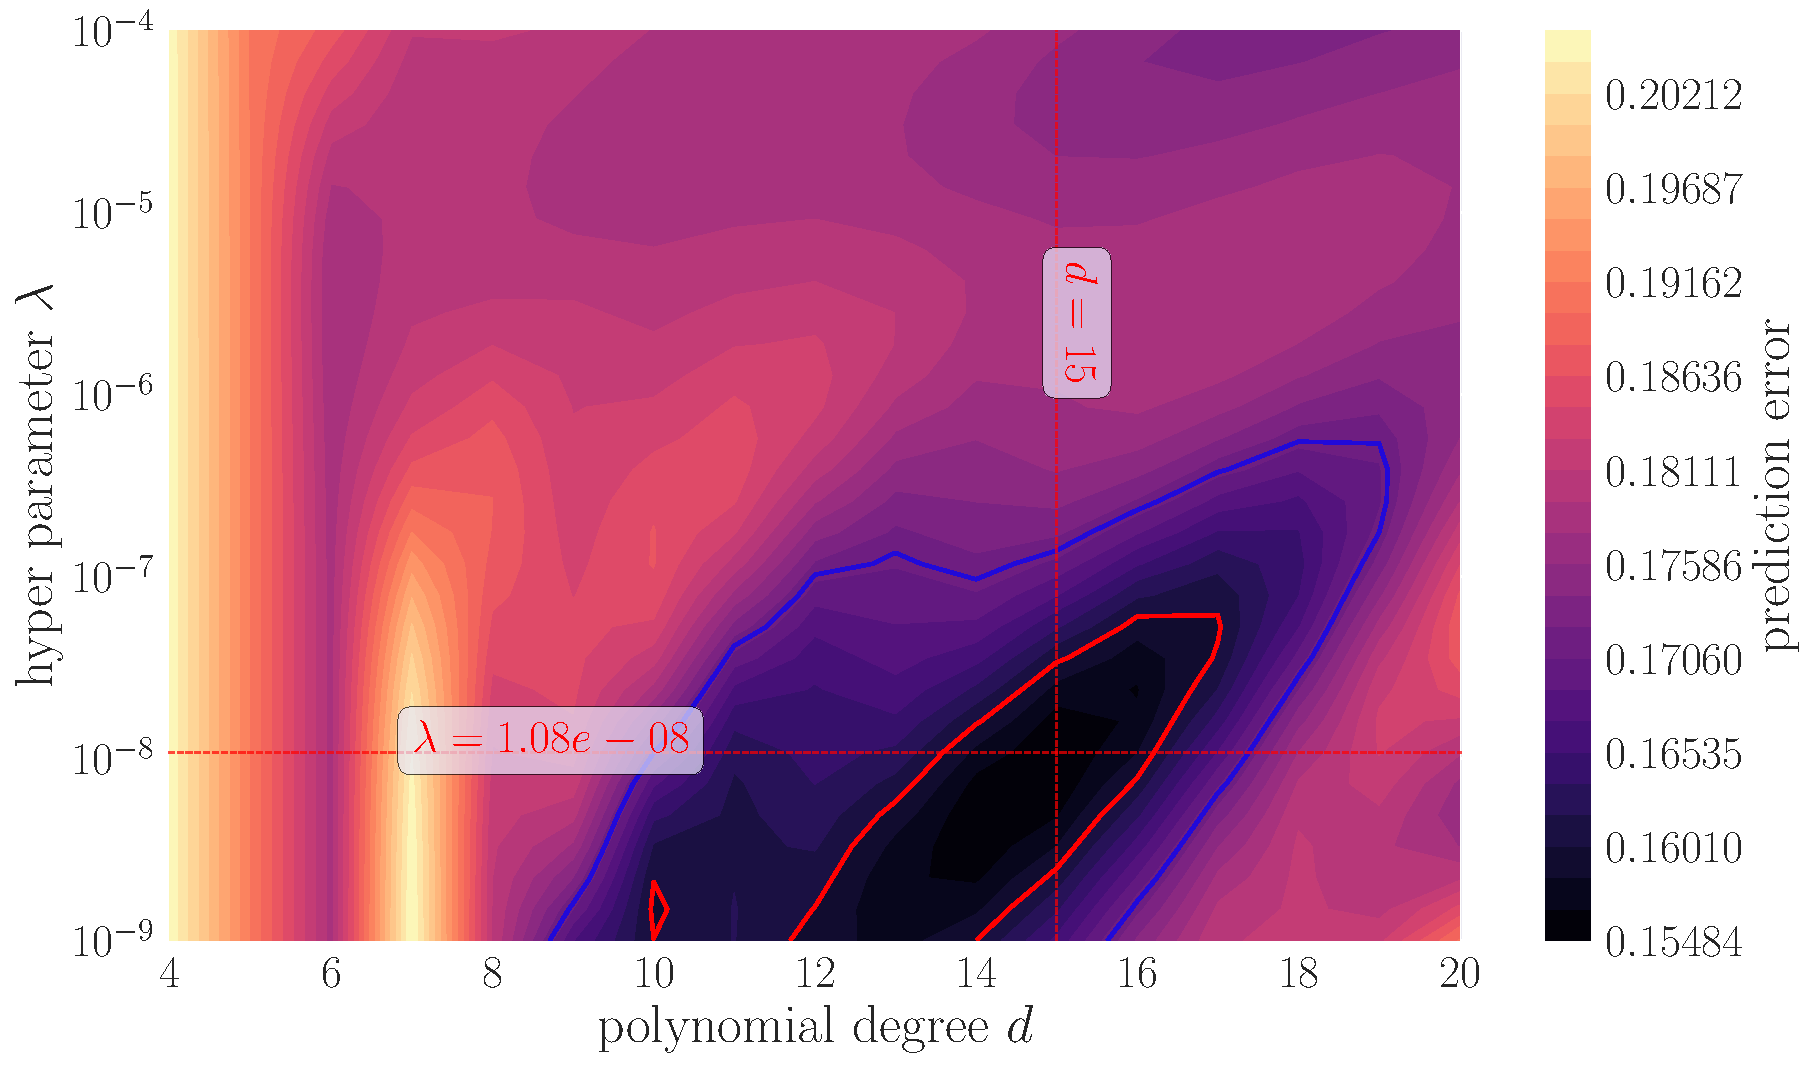
\includegraphics[width=\linewidth]{terrain/MSE_heatmap_ridge_CV.pdf}
            \caption{Heatmap of the prediction MSE as function of both polynomial degree $d\in[4,20]$ and penalty parameter $\lambda$ for the ridge analysis of the terrain data, generated with a 10-fold cross validation. Parameters yielding minimum MSE are shown in the figure. }
            \label{fig:gc_gridsearch_ridge}
        \end{figure}

        The error heatmap in \Fig{gc_gridsearch_ridge} favourises the combination $d=18, \lambda = 1.23\cdot 10^{-4}$. In an attempt to verify this model, we do the bootstrap for this polynomial degree and the same hyper parameters. The resulting train and test MSE is shown in \Fig{gc_model_complexity_ridge}.

        \begin{figure}
            \includegraphics[width=\linewidth]{terrain/MSE_ridge_BS.pdf}
            \caption{MSE for train and test data fo polynomial of degree $d=18$ as a function of the penalty parameter $\lambda$ for the ridge analysis of the terrain data, $k=400$ bootstrap. }
            \label{fig:gc_model_complexity_ridge}
        \end{figure}

        We investigate the bias-variance tradeoff by the same bootstrap session. The tradeoff is shown in \Fig{gc_bias_variance_ridge}. It shows nothing to indicate precisely which hyper parameter is best, but it does not contradict the model found by the grid search.

        \begin{figure}
            \includegraphics[width=\linewidth]{terrain/tradeoff_ridge.pdf}
            \caption{Bias variance and residual error for polynomials degree $d=18$ as function of the penalty parameter $\lambda$ for the ridge analysis of the terrain data, generated with a $k=400$ bootstrap.}
            \label{fig:gc_bias_variance_ridge}
        \end{figure}

        There are actually models with $d=15\pm 1, \lambda\sim  10^{-8}$ which give cross-validation accuracy $\lesssim 0.16$ for various choices of $k$. However, when confirming these models using bootstrap, the prediciton errors grow huge, as do both the variance and squared bias, in the regime of $\lambda\sim 10^{-8}$. There is a sudden drop in error and variance for $\lambda \simeq 8.5 \cdot 10^{-9}$ for $d=15$, but this now seems random.


        \subsubsection{Lasso}\label{sec:gc_lassoanalysis}

        The same strategy is used with Lasso regression. This is much more frustrating as the computational expenses of minimising the Lasso cost function are much higher than for the two others. A grid search indicates that we need $\lambda \geq 10^{-5}$ for $d=11$ in order to get cross-validation generalisation errors down to $0.19$. This is illustrated in \Fig{gc_gridsearch_lasso}.

        \begin{figure}
            \includegraphics[width=\linewidth]{terrain/MSE_heatmap_lasso_CV.pdf}
            \caption{Heatmap of the prediction MSE as function of both polynomial degree $d\in[4,20]$ and penalty parameter $\lambda$ for the Lasso analysis of the terrain data, generated with a 10-fold cross validation. Parameters yielding minimum MSE are shown in the figure.}
            \label{fig:gc_gridsearch_lasso}
        \end{figure}

        There is little point in continuing with validation of this model. In this paper, we omit the rest of the Lasso analysis due to 

        \begin{enumerate}[label=(\roman*)]
            \item the computational expense of the bootstrap and Lasso algorithm combined is very large, and even larger for smaller $\lambda$'s, and
            \item a wish to reduce the number of figures for the sake of a legibility.
        \end{enumerate}

      





    